%
% chapter3.tex
%

\chapter{NVIDIA Bluefield-3}
\label{cha:design}
Die im Rahmen dieser Arbeit verwendete SmartNIC ist die von Nvidia im Jahre 2022 veröffentlichte Bluefield-3. Wie bereits am Namen der Karte zu erkennen ist, handelt es sich dabei um die dritte Generation von Netzwerkkarten, die zusätzlich zur netzwerkspezifischen Architektur noch einen allgemeinen ARM-Prozessor verbaut hat. Zusätzlich wird in einem späteren Abschnitt ein Überblick über das DOCA-Framework gegeben, welches von NVidia als einheitliche Programmierschnittstelle veröffentlicht wurde, um die Programmierung der Hardware von der jeweiligen Generation unabhängig zu machen.
\section{Entstehung}
Die Entwicklung der BlueField ist ein Produkt der letzten Dekade, in der ein immerwährend größeres Interesse an der Effizienzsteigerung von Rechenzentren entstanden ist. Energiesparende Systeme, die dieselbe Leistung erreichen wie selbige Integration auf einem allgemeinen Prozessor, bieten für Systemintegratoren eine ausgezeichnete Möglichkeit, auch vor dem Hintergrund des Klimawandels energieoptimierte Systeme zu entwickeln.
\subsection{BlueField-1}
Die erste Generation der Bluefield-Hardware wurde im Jahre 2017 von Mellanox Technologies vorgestellt und bildet den ersten Eintrag in die Reihe der Bluefield-SmartNIC-Serie. Sie kombinierte erstmalig die ConnectX-5-Plattform mit einem ARM-basierten System-on-Chip. Die Idee dahinter war es, das Verhalten der Netzwerkplattform mittels User-Anwendungen beeinflussen zu können. Dazu wurde eine API zwischen der ConnectX und dem ARM-Prozessor entwickelt. Hierzu sei erwähnt, dass es sich bei der ConnectX-Plattform um eine bereits weit verbreitete und in viele Systeme integrierte Hardware handelte. Sie besaß bereits zum damaligen Zeitpunkt eine breite Anzahl von paketbasierten Operationen, mit deren Hilfe eine weitreichende Manipulation sowie Paket-Steering oder anderweitige Verwendungen ermöglicht wurden. Die BlueField-1 war mit einem ARM-A72 mit 4 Kernen und 8 Threads ausgestattet und besaß außerdem zwei QSFP28-Anschlüsse, welche bis zu 100 Gbps Durchsatz erreichen konnten. Die Zielgruppe der BlueField-Serie war von Anfang an der Enterprise-Markt sowie die zahlreichen größeren Rechenzentren, in denen Rechenoperationen ausgeführt werden, die auf mehreren Computern eines Clusters oder einer Clusterstruktur ausgeführt werden. Gerade in diesem Umfeld wird eine derartige Architektur von Interesse, da der Netzwerkverkehr so anwendungsspezifischer verteilt werden kann und somit die Effizienz eines Rechnerverbundes steigern kann. 
\begin{figure}
    \centering
    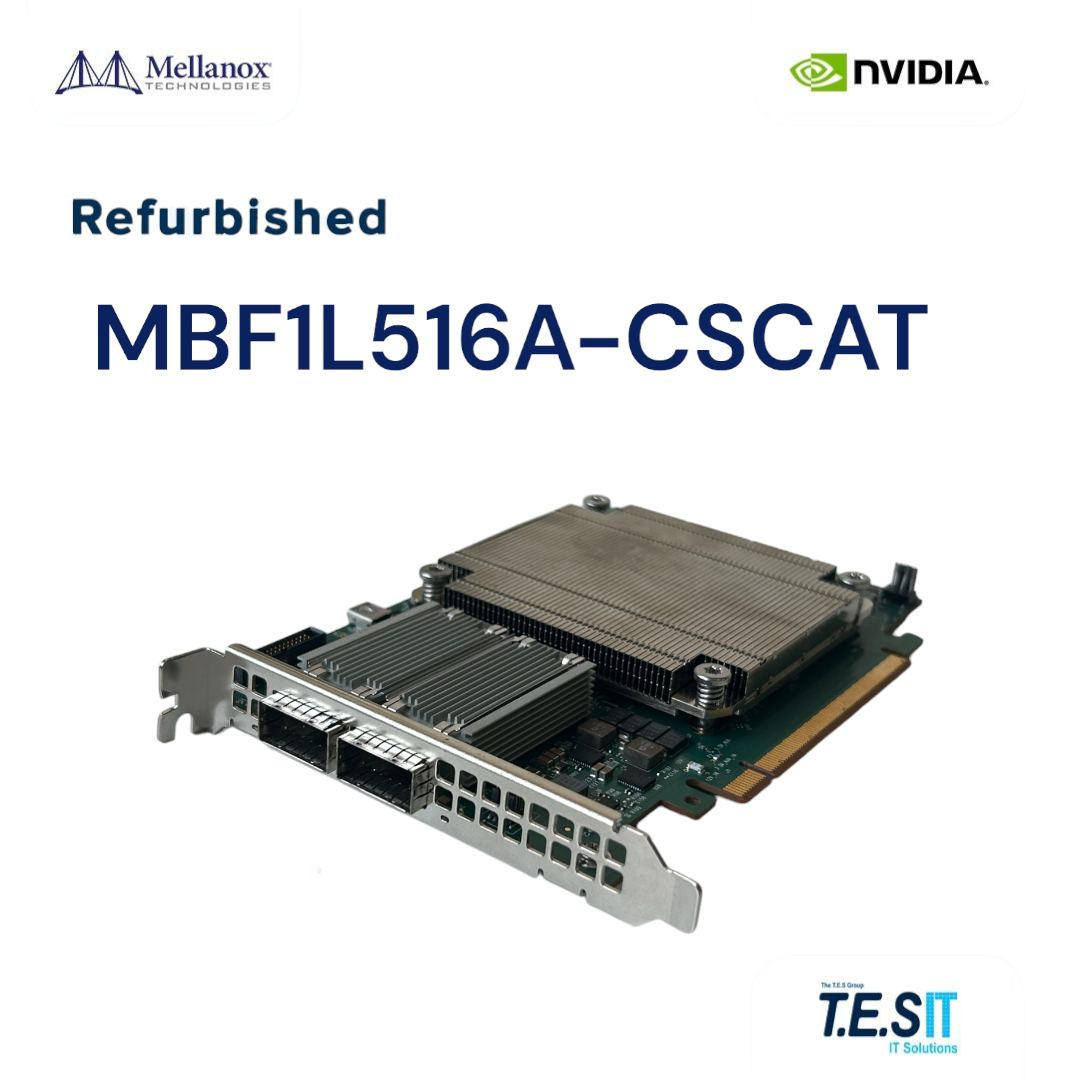
\includegraphics[width=0.65\linewidth]{images/s-l1600.png}
    \caption{BlueField-1 Karte}
    \label{fig:enter-label}
\end{figure}
\subsection{BlueField-2}
Nach der Übernahme von Mellanox durch den Chip-Hersteller NVIDIA im Jahre 2019 wurde das Projekt BlueField von NVIDIA nicht nur weitergeführt, sondern mit dem Aufkommen von vermehrten Machine Learning Workloads sogar das Marketing ausgebaut. So wurde die BlueField-2 im Jahre 2021 unter dem neuen Hersteller NVIDIA veröffentlicht und bot nun einen QSFP56, der laut eigenem Marketing-Material bis zu 200 Gbps erreichen sollte. Abermals kam der ARM A72 zum Einsatz, der erneut mit 4 Kernen und 8 Threads verbaut wurde. Erstmalig wurde außerdem damit geworben, dass ein Einsatz in Machine-Learning-Rechenclustern besonders wertvoll sei. Auf genauere Angaben, warum genau, wurden seitens des Herstellers bisher nicht erbracht. Insbesondere nicht vor dem Hintergrund, warum es sich dabei nun um ein Alleinstellungsmerkmal anderen SmartNICs gegenüber handeln sollte.
\subsection{BlueField-3}
Zuletzt wurde im Jahre 2022 die BlueField-3 veröffentlicht, die im Rahmen dieser Arbeit zur Verwendung kam. Erstmalig wurde nun der ARM-A78 mit 8 Kernen und somit 16 Threads verbaut. Die Arbeitsspeicherarchitektur nahm zusätzlich auch den Generationensprung von DDR4 auf DDR5 und verwendet so deutlich schnelleren Speichertakt als die vorherige Generation. Außerdem wurde erneut der Netzwerkanschluss aktualisiert und verwendet nun den QSFP112. Laut NVIDIA soll mit diesem Netzwerkverbund eine Line Rate von bis zu 400 Gbps erreicht werden. Dabei wird im Marketing-Material nicht explizit erwähnt, welche Paketgröße für besagten Durchsatz verwendet wurde. Erneut soll laut NVIDIA der Fokus der Hardware vermehrt auf dem Einsatz in Rechenzentren liegen, in denen größere Machine-Learning-Lasten laufen. Die BlueField-3 soll daraufhin die Rolle einer intelligenteren Paketverteilung einnehmen, wobei die Last der Lastverteilung nicht mehr auf dem Hostsystem bzw. dem entsprechenden Host-Prozessor liegen, sondern eben auf der Netzwerkkarte selbst. Außerdem sind eine Menge von weiteren speziellen hardwarebeschleunigten Hardwareeinheiten auf der neuesten Iteration der BlueField-Serie verbaut worden. Alle genannten Generationen BlueField werden per PCI-E Stecker in den Hostsystemen verbaut und verwenden so den aktuellsten PCI-E 5.0 Standard, der auf eine theoretische Maximalbandbreite von 32 Giga Transfer/s kommt. Somit soll eine ultraschnelle Schnittstelle zwischen Hostsystem und BlueField-3 erreicht werden.
\section{Architektur}
Um der Funktion einer intelligenten Netzwerkkarte nachzukommen, sind auf der BlueField diverse Hardwareeinheiten verbaut, die eine Reihe von Einsatzzwecken abdecken sollen. Dabei werden nicht alle angebotenen Funktionen auch tatsächlich von ASIC-Hardwareeinheiten übernommen, sondern werden teilweise komplett oder nur in bestimmten Pipeline-Abschnitten auf dem ARM Core ausgelagert, um dort einer weiteren Behandlung unterzogen zu werden. Wie in Abbildung 3.2 zu erkennen ist, gliedert NVIDIA die BlueField-Karte grob in Domänen unterschiedlichster Funktion auf. Abgesehen vom ARM-Teil der Karte, womit im Wesentlichen der Bereich beschrieben wird, in dem der Prozessor, Arbeitsspeicher und restlicher I/O zusammengefasst werden, sind die beiden Bereiche \textbf{Accelerators} und \textbf{Accelerated Programmable Pipeline} diejenigen, in denen eine große Menge der eigentlichen Hardwarebeschleuniger sitzen. Allerdings geht aus dem von NVIDIA bereitgestellten Material nicht vollständig hervor, worum es sich bei dem sogenannten Datapath Accelerator handelt. Im Release-Flyer der BlueField-3 steht allerdings, dass es sich dabei auch um einen Prozessor mit 16 Kernen handeln soll, der mit 256 Threads ausgestattet ist. Dies würde bedeuten, dass jeder Kern von Hause aus 16 Threads besitzt. Zusätzlich wird oft darauf verwiesen, wie einfach ein Zusammenspiel von DPU und Hostsystem mittels der PCI-E Anbindung funktionieren soll. Laut Hersteller werden in den oben genannten Bereichen folgender Ausschnitt von Beschleunigern und Funktionen angeboten. 
\begin{figure}
    \centering
    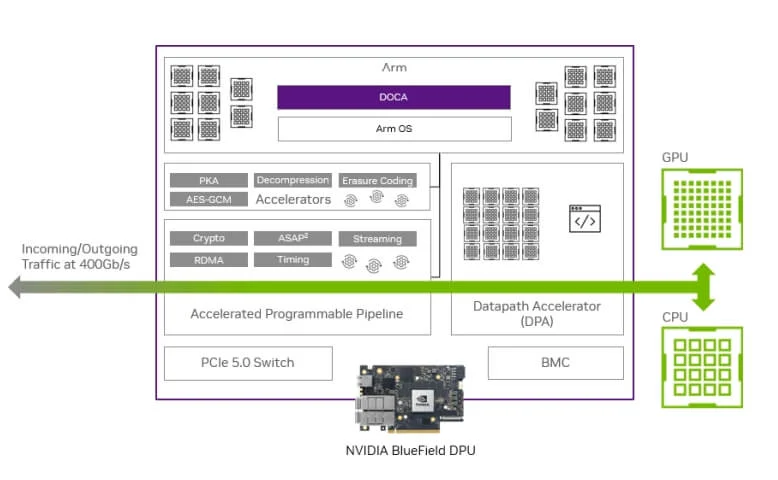
\includegraphics[width=1\linewidth]{images/nvda-bluefield-dpu.png}
    \caption{BlueField-3 Architektur}
    \label{fig:enter-label}
\end{figure}
\subsection{Hardwareeinheiten}
\subsubsection{PKA}
PKA steht für Public-Key-Acceleration und bietet eine Reihe von Funktionalitäten im Zusammenhang mit der Arbeit mit öffentlichen Schlüsseln im Kontext von SSL-Anwendungsfällen. So stellt es beispielsweise einfache bis komplexere arithmetische Operationen wie RSA, Diffie-Hellman sowie Addition und Subtraktion bereit. Es soll eine einfache Programmierschnittstelle bieten, sobald die DOCA-Applikation mit Verschlüsselungen hantiert, die möglichst schnell umgesetzt werden sollen.
\subsubsection{Decompression}
Die Dekompressionsbeschleuniger der BlueField-3 sollen vor allem dann zum Tragen kommen, wenn die Netzwerkkarte mit Buffern konfrontiert wird, in denen die Daten komprimiert vorliegen. Dabei soll sich diese möglichst nicht auf die Verarbeitung des Datenverkehrs auswirken.
\subsubsection{Erasure Coding}
Erasure Coding bezeichnet die Hardwareeinheit, deren hauptsächliche Funktion die forward error correction ist. Dies wird dazu verwendet, um eventuelle Übertragungsfehler oder umgedrehte Bits mithilfe der Paritätsinformation reparieren zu können.
\subsubsection{AES-GCM}
AES ist ein bekannter Verschlüsselungsstandard, der quasi von jedem Endgerät dieser Welt implementiert wird, um modernen Sicherheitsanforderungen gerecht zu werden. Hierzu hat NVidia eine Hardwareeinheit entwickelt, um Daten auch im eigenen Arbeitsspeicher verschlüsseln zu können.
\subsubsection{RDMA}
RDMA ist die Abkürzung für Remote Direct Memory Access. Innerhalb eines solchen Prozesses kann ein Prozess auf den Speicherbereich eines anderen Rechners zugreifen. Damit wird eine Alternative zum klassischen Netzwerkverkehr angeboten.
\subsection{Datapath Accelerator}
Der Datapath Accelerator, kurz DPA, ist für diese Arbeit von besonderem Interesse, da laut NVidia hier ein Großteil der Netzwerkverarbeitung vorgenommen wird. Wie bereits im vorherigen Kapitel zum Hardwareaufbau erwähnt, soll hier ein weiterer Prozessor zum Einsatz kommen, der über ein extremes 16-faches Multithreading verfügt. Dieses Multithreading wird benötigt, um möglichst latenzfreie Verarbeitung umzusetzen. Leider sind seitens des Herstellers allerdings keine weiteren Angaben zur verbauten Hardware freigegeben worden. Daher ist es ohne weitere Informationen nicht möglich, die genauere Funktionsweise zu analysieren. Dennoch sollte es, sofern es sich dabei denn wirklich um den trafficverarbeitenden Prozessor handelt, in den späteren Messungen zu beobachten sein, dass der ARM-Prozessor von dem eingehenden Verkehr unberührt bleiben sollte.

\section{DOCA Framework}
DOCA ist ein von NVidia entwickeltes Framework, das speziell für die BlueField-Karten entwickelt wurde. Es gliedert sich in verschiedene Teilbereiche und unterscheidet dabei zwischen architektonischen Grundsätzen, Programmierinterfaces, aber auch dem Betriebssystem für die Karte selbst. Allgemein ist DOCA dafür gedacht, der direkte Anlaufpunkt für Entwickler zu sein, die auf der BlueField-Plattform entwickeln wollen. Damit werden auch Dinge wie Programmiersprachen, Programmierparadigmen und eine Reihe von bereits angelegten Bibliotheken bereitgestellt. Zusätzlich werden sämtliche Hardware-Treiber ebenfalls unter dem Oberbegriff DOCA zusammengefasst. Im Folgenden wird ein Überblick zu DOCA im Allgemeinen gegeben und ein besonderes Augenmerk auf die für diese Arbeit relevanten Teilbereiche gelegt.
\begin{figure}
    \centering
    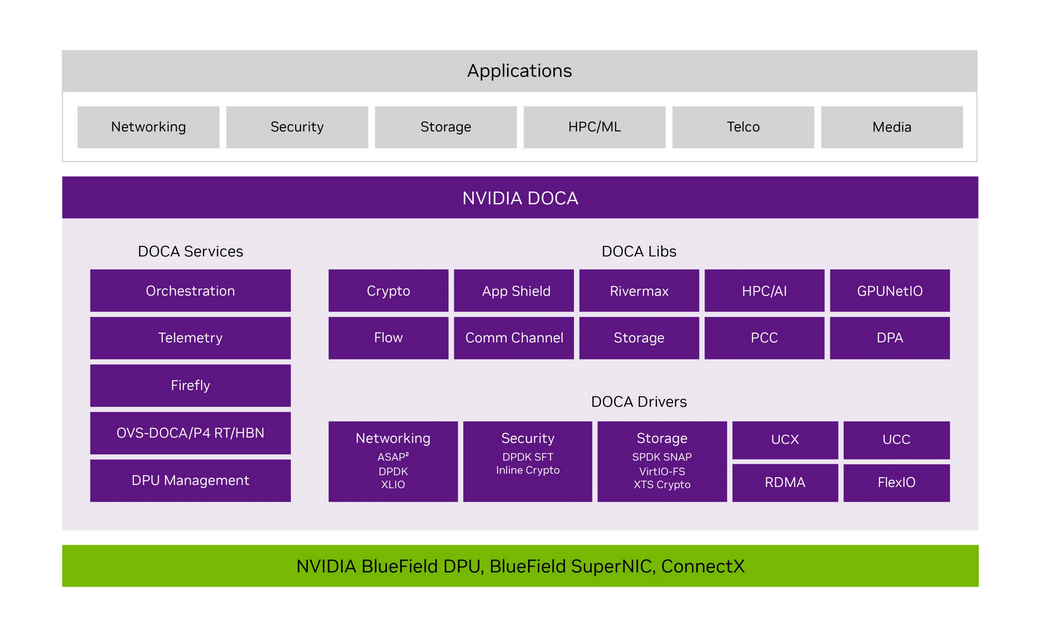
\includegraphics[width=1\linewidth]{images/Screenshot 2025-04-26 at 08-31-41 DOCA Overview - NVIDIA Docs.png}
    \caption{Überblick der Teilbereich von DOCA}
    \label{fig:enter-label}
\end{figure}
\subsection{DOCA Services}
DOCA stellt eine Reihe von Services bereit, die vorrangig dazu dienen sollen, eine Ende-zu-Ende-Lösung für einen speziellen Anwendungsfall zu bieten. Dazu gliedert NVidia diverse (Abbildung 3.3) Unterkategorien aus. Einerseits aufgrund des primären Anwendungsfeldes in Rechenzentren wird viel Wert auf Orchestrierung gelegt. Leider bleibt NVidia hier bemerkenswert ungenau, was genau damit eigentlich gemeint ist. Bei der Telemetrie hingegen stellt NVidia eine große Schnittstelle bereit, um genaue hardwarebezogene Daten abrufen zu können. Hierzu werden den Entwickelnden zwei Tools bereitgestellt. Das Tool \textbf{doca\_telemetry\_diag} stellt die Konfiguration des Loggings dar. Dazu kann mithilfe besagter Tools festgelegt werden, welche Telemetriedaten erhoben werden sollen und auch in welchem Samplingintervall. Diese Daten können dann in diversen auswählbaren Dateiformaten abgerufen werden. \textbf{doca\_telemtery\_pcc} soll den Zugang zu speziellen algorithmischen Daten ermöglichen. Damit sind die bereits in DOCA vorimplementierten Funktionen gemeint, die meist hardwarebeschleunigt, also außerhalb des sichtbaren Bereichs des ARM-Hosts, ausgeführt werden. Sonstige Services wie beispielsweise der Firefly sind NVidias Implementierungen des Precision Time Protocols. Ziel dieses Protokolls ist es, die Zeit innerhalb eines Clusters möglichst genau propagieren zu können. Dazu verspricht NVidia, möglichst viel von dieser Komplexität vor dem Anwender mithilfe von Firefly fernzuhalten. Außerdem setzt NVidia zur Konfiguration des Datenverkehrs stark auf die Integration von Open vSwitch (OVS). Dazu wurde eigens ein eigener Service entwickelt, der abermals die eigentliche Komplexität des Konfigurationsprozesses dem Entwickler abgenommen werden soll. Hauptgrund ist allerdings vermutlich, dass, um mit den spezifischen Hardwareeinheiten überhaupt kommunizieren zu können, die Open vSwitch-Interfaces angepasst werden müssen. 
\subsection{DOCA Bibliotheken}
Damit eine reibungslose Inbetriebnahme sowie Programmierung einer SmartNIC erfolgen kann, muss klar definiert sein, wie, sofern programmatische Konfigurationen erfolgen sollen, ein Entwickler mit der entsprechenden Hardwareeinheit kommunizieren kann. Damit ist es nicht mehr nötig, die Feinheiten der einzelnen Hardwarekommunikationskanäle zu implementieren, sondern es kann auf eine mehr oder weniger vereinheitlichte Programmierschnittstelle zugegriffen werden. Dazu stellt NVidia Programmbibliotheken in Form von C-Headern bereit, mithilfe derer intrinsische Funktionen auf der Architektur ausgeführt werden können. Dabei lässt sich grob formulieren, dass jede in Kapitel 3.2.1 genannte Hardwareeinheit eben auch eine entsprechende Bibliothek bekommen hat. Zusätzlich gibt es aber auch Bibliotheken, die Funktionen wie Speicherverarbeitung für Anwendungsfälle wie verteilte Speichersysteme implementieren.
\subsubsection{DOCA Flow}
DOCA Flow ist die Bibliothek, die sich vollständig mit der Verarbeitung und Modifikation von Netzwerkpaketen beschäftigt. Das Versprechen seitens NVidia ist hierbei, dass alle Funktionen von Flow auf den Hardwarebeschleunigern ausgeführt werden können. DOCA Flow wird, wie viele moderne Systeme, deklarativ programmiert. Das bedeutet, der State des aktuellen Netzwerkverkehrs ist immer genau so, wie er durch die Konfiguration deklariert wurde. Dies hat den großen Vorteil, dass die Entwicklung und in der Folge auch das Debugging sich immer direkt mit dem Programmcode selbst befassen kann, da keine Fehler zur Laufzeit entstehen können (sollten) die so nicht klar vorher definiert worden sind.
\subsection{DOCA Treiber}
\subsection{Anwendungen}
